\documentclass[tikz]{standalone}

\usepackage{tikz}
\usetikzlibrary{matrix, positioning, fit, shapes, decorations.pathreplacing}


% see http://www.texample.net/tikz/examples/colorful-tables/
% see http://tex.stackexchange.com/questions/1111/problem-with-defining-shortcuts-for-tikz-matrices

\newcommand{\connectionsMatrix}[2][]{
  \def\x{$\bullet$}
  \matrix (#2) [#1, matrix of nodes, nodes in empty cells,
    ampersand replacement=\&,
    column sep=0pt, row sep=0pt, inner sep=0pt,
    nodes={ draw, color=lightgray, text=black, minimum size=1cm, anchor=center },
    column 1/.style={nodes={draw=none}},
    row 1/.style={nodes={draw=none}},
    ]{
         \& $p_1$ \& $p_2$ \& \dots \& $p_k$ \& \dots \& \dots \& $p_m$ \\
  $g_1$  \&       \&   \x  \&       \&       \&   \x  \&       \&   \x  \\
  $g_2$  \&   \x  \&       \&   \x  \&       \&   \x  \&   \x  \&       \\
  \vdots \&       \&   \x  \&       \&       \&   \x  \&   \x  \&       \\
  $g_i$  \&   \x  \&       \&   \x  \&   \x  \&       \&       \&       \\
  \vdots \&       \&       \&   \x  \&       \&   \x  \&       \&   \x  \\
  $g_n$  \&   \x  \&       \&       \&   \x  \&       \&   \x  \&   \x  \\
  };
}

\def\mminh{2}
\def\mmaxh{8}

\def\mminv{2}
\def\mmaxv{7}

\def\mmin{\mminh}
\def\mmax{\mmaxh}

% matrix, row, color
\newcommand*{\fith}[4][]{
  \def\m{#2}
  \def\i{#3}
  \def\color{#4}
  \node[fit=(\m-\i-\mmin) (\m-\i-\mmax), inner sep=-5pt, draw, color=\color, #1] {};
}

% matrix, column, color
\newcommand*{\fitv}[4][]{
  \def\m{#2}
  \def\j{#3}
  \def\color{#4}
  \node[fit=(\m-\mminv-\j) (\m-\mmaxv-\j), inner sep=-5pt, draw, color=\color, #1] {};
}


\newcommand{\used}[4]{
  \def\m{#1}
  \def\r{#2}
  \def\c{#3}
  \def\color{#4}
  \node[draw, cross out, color=\color, inner sep=5pt, thick] at (\m-\r-\c) {};
}
\newcommand{\usedv}[3]{\used{#1}{1}{#2}{#3}}
\newcommand{\usedh}[3]{\used{#1}{#2}{1}{#3}}


\begin{document}

\newcommand*{\mkCandidate}[6][]{
  \def\g{#2}
  \def\n{#3}
  \def\ps{#4}
  \def\r{#5}
  \def\color{#6}

  \node[group, #1, color=\color] (G-\g) {$g_\g$};

  \edef\a{-45}
  \pgfmathsetmacro{\da}{135/\n}%
  \foreach \p in \ps {
    \path (G-\g) -- ++(\a:\r) node[prof] (P-\p) {$p_\p$};
    \draw[-, color=\color] (G-\g) -- (P-\p)
          node [midway, class, fill=red, color=black] {};
    \pgfmathparse{\a+\da}
    \global\edef\a{\pgfmathresult}
    }
}


\newcommand*{\showCandidate}[7]{
  \def\m{#2}
  \def\i{#3}
  \node[fit=(\m-\i-\mmin) (\m-\i-\mmax), inner sep=-5pt, draw, color=#1] {};
  \mkCandidate[right=#5 of \m-\i-\mmax] {#4}{#6}{#7}{2cm}{#1}
}


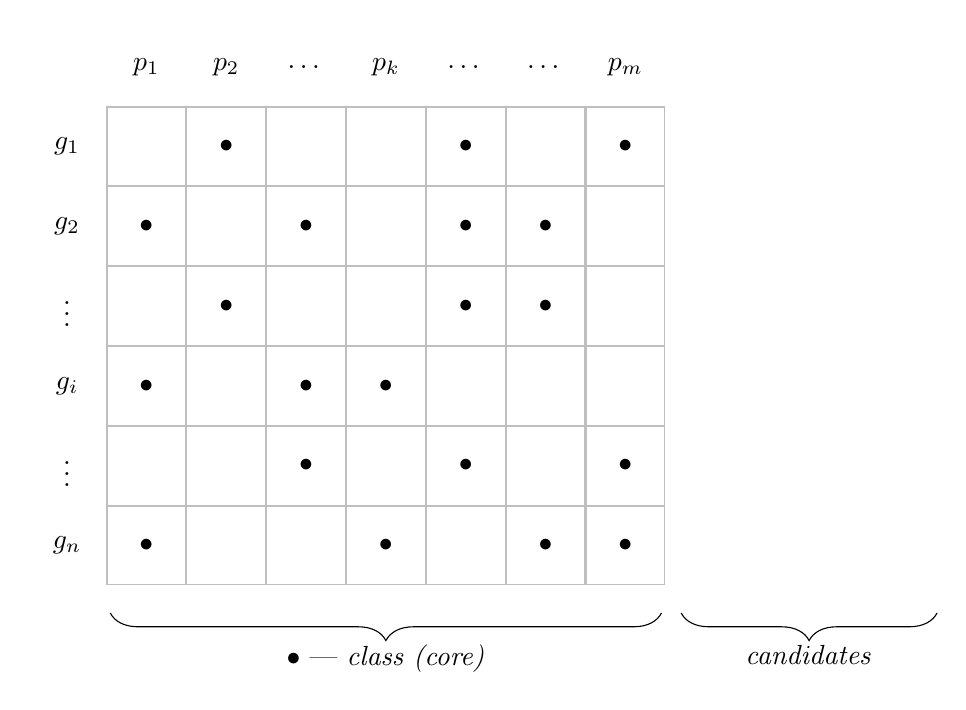
\begin{tikzpicture}

% Matrix - Candidates
\connectionsMatrix{m};
\begin{scope}[
  scale=0.5,
  agent/.style={draw, minimum size=0.5cm, inner sep=1pt, font=\small},
  group/.style={agent, diamond},
  prof/.style={agent, circle},
  class/.style={draw, circle, fill, inner sep=1pt},
  ]

  \showCandidate{blue}           {m}{2}{1}{5pt}  {3}{2, *, m}
  \showCandidate{green!50!black} {m}{3}{2}{1.7cm}{4}{1, *, *, *}
  \showCandidate{orange!50!black}{m}{4}{*}{5pt}  {3}{2, *, *}
  \showCandidate{blue}           {m}{5}{i}{2cm}  {3}{1, *, k}
  \showCandidate{green!50!black} {m}{6}{*}{5pt}  {3}{*, *, m}
  \showCandidate{orange!50!black}{m}{7}{n}{1.7cm}{4}{1, k, *, m}

  \draw [decorate,decoration={brace,amplitude=10pt,mirror,raise=4pt}]
        (-6,-7.5) -- node[below=12pt]{$\bullet$ --- \emph{class (core)}} (8,-7.5);

  \draw [decorate,decoration={brace,amplitude=10pt,mirror,raise=4pt}]
        (8.5,-7.5) -- node[below=12pt]{\emph{candidates}} (15,-7.5);

\end{scope}


\end{tikzpicture}

\end{document}
